\documentclass{article}
\usepackage{color}
\usepackage{xcolor}
\usepackage{amsmath}
\usepackage[thinlines]{easytable}
\usepackage{graphicx}
\usepackage{enumitem}
\usepackage{listings}

% Tikz stuff
\usepackage{tikz}
\usepackage{tikz-qtree}
\usepackage{tikz-qtree-compat}
\usetikzlibrary{positioning}

\tikzset{blue node/.style={circle,fill=blue!20,draw,minimum size=1cm,inner sep=0pt},}
\tikzset{red node/.style={circle,fill=red!20,draw,minimum size=1cm,inner sep=0pt},}
\tikzset{green node/.style={circle,fill=green!20,draw,minimum size=1cm,inner sep=0pt},}
\tikzset{yellow node/.style={circle,fill=yellow!20,draw,minimum size=1cm,inner sep=0pt},}

\tikzset{graph node/.style={circle,fill=orange!30,draw,minimum size=1cm,inner sep=0pt},}

\title{COS 485 --- Homework 5}

\author{Samuel Barton \and Benjamin Montgomery}

\date{April 3, 2017}

\begin{document}
	\maketitle
	\section*{Problem 1}

In this problem we categorize the following sorting algorithms into the
various genres of algorithms discussed in this course.
\\
\\
By definition, iterative improvement gradually improves an initial solution.
Thus it is impossible for a sorting algorithm to be an iterative improvement 
algorithm as a list is either sorted or unsorted. Once there is a solution,  no
improvements can be made on it.
\\
\\
\begin{tabular}{l c p{6cm}}
        \textbf{Algorithm} & \textbf{Technique} & \textbf{Justification} \\
        \hline
    Insertion sort & Greedy & Go through each element starting at position 0. Shift all of the elements greater than the current one to the left.\\
    Selection sort & Greedy & Find the smallest item in the unsorted part of the list and append it to the end of the sorted part. \\
    Bubble sort & Greedy & If the next value is smaller than the current one, swap them.\\
    Quicksort & Divide and Conquer & Divide the problem size recursively, sort at the bottom, then sort on your way up. Note that Quicksort \textit{can} be implemented with a randomized partition.\\
    Merge sort & Divide and Conquer & Divide the problem size recursively, sort at the bottom, then sort on your way up.\\
    Heap sort & Greedy & Larger values go higher (maxheap), or smaller values go higher (minheap)\\
\end{tabular}

	\section*{Problem 2}

We are given two problems $A$, $B$, such that $A$ can be converted to $B$ in $t_n \in \Theta(n^3)$, meaning $A \propto B$ if the solution to $B$ has $t_n \in \Theta(n^b)$, a polynomial quantity. To bound the complexity of this solution, we will refer to the below proof:

\begin{proof}
Suppose we have an instance of problem $A$ that is of size $n$. Because at most there are $\Theta(n^3)$ steps in the transformation algorithm, and at worst the algorithm outputs a symbol at each step, the size of the instance of $B$ produced by the transformation is at most a quantity $s$ such that $s \in \Theta(n^3)$. When that instance is the input to the algorithm for $B$, this means there are at most $\Theta\left((n^3)^b\right)$ steps. Therefore, the maximum number of work required to transform the instance of problem $A$ to an instance of problem $B$ and then solve problem $B$ to get the correct answer for problem $A$ is at most
$$
\Theta(n^3) + \Theta\left((n^3)^b\right)
$$
which is a polynomial in $n$.
\end{proof}

	\pagebreak
	\section*{Problem 3}

In this problem we explain a way the algorithm in Exercise 5.19 could be implemented.

\begin{lstlisting}
Let there be an array where we will store the colors we create

Let there be an adjacency list for this graph

Let there be a count of uncolored nodes

for each node in the adjacency list
    if the count of uncolored nodes is zero
        stop
    if the node has not been colored
        pick a new color
        add that color to the array of possible colors
        color that index with the new color
        decrement the count of uncolored nodes
        for each node in the adjacency list
            if this node is not adjacent to any nodes with the current color 
                color this node
                decrement the count of uncolored nodes
\end{lstlisting}

Using the above implementation, the algorithm would take the following amount of time for an arbitrary graph with N nodes.
\\
\\
The outermost loop will iterate N times in the worst case, thus in the worst case we will have N colors. This would happen if we were handed a completely connected graph. Our algorithm visits each node in the graph, and at each node, it then visits every other node in the graph. Thus, our traversal requires $\Theta(N^2)$ operations; however, at each of these visits, we must perform an $O(N)$ adjacency check in order to determine if we should color that node. This means we have, based on experience, an $\mathrm{O(}N^3 \mathrm{)}$ algorithm in the worst case. 
\\
\\
Since we wish for a more instructive analysis of this algorithm, we are going to analyze at a higher level of granularity. Thus, we may note that the number of times we go through the outer loop is dependent on the number of colors needed to completely color the graph. The number of colors needed is dependent on the level of connectedness in the graph. Thus, if it takes K colors to completely color the graph, then our algorithm is  $\mathrm{\Theta (}K \cdot N^2 \mathrm{)}$. 
	\pagebreak
	\section*{Problem 4}

In this problem we are asked to demonstrate the use of our greedy algorithm from Problem 3 to color the graph shown below. Interestingly, the algorithm does indeed produce an optimal coloring for the graph as there is no possible way to get a coloring with only two colors given the extra edge between nodes 5 and 7.

\begin{center}
    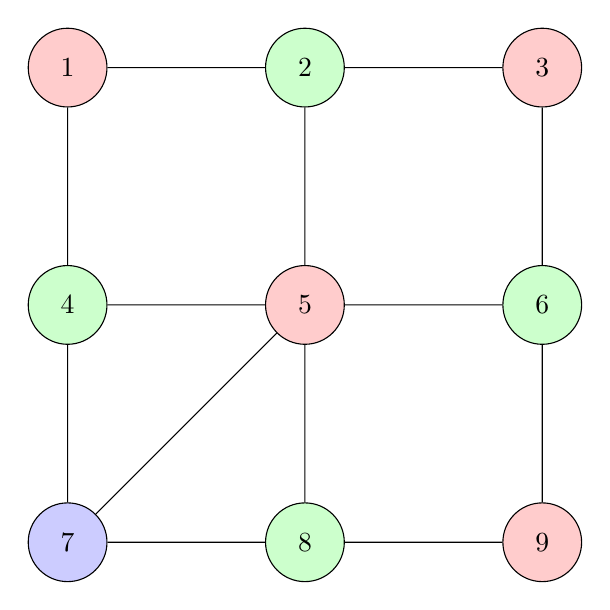
\begin{tikzpicture}
       \node[red node] (1) {$1$};
       \node[green node] (2) [right = 2cm of 1]{$2$};
       \node[red node] (3) [right = 2cm of 2]{$3$};
       
       \node[green node] (4) [below = 2cm of 1]{$4$};
       \node[red node] (5) [right = 2cm of 4]{$5$};
       \node[green node] (6) [right = 2cm of 5]{$6$};
       
       \node[blue node] (7) [below = 2cm of 4]{$7$};
       \node[green node] (8) [right = 2cm of 7]{$8$};
       \node[red node] (9) [right = 2cm of 8]{$9$};
       
       \draw
       (1) -- (2) -- (3)
       (1) -- (4) -- (7)
       (2) -- (5) -- (8)
       (3) -- (6) -- (9)
       (4) -- (5) -- (6)
(7) -- (8) -- (9)
       (7) -- (5);
    \end{tikzpicture}
\end{center}

	\section*{Problem 5}

The following is an an algorithm for finding the mode in an unsorted array so large we can't do anything fun, like using HashMaps.
\begin{enumerate}
    \item Pivot using a random pivot. Move information around like in Quick Select.
    \item Keep track of how many times the pivot occurs. Store this pivot value and count to one side.
    \item Compare the cardinality of the subset of items equal to the pivot value with the cardinality of the sets of vales to the right and to the left of it.
    \begin{enumerate}
        \item If the right of the pivot is larger than the cardinality of the pivot, recursively repeat this process on the right side. Mirror case for the left.
        \item If the cardinality of the pivot is the largest, then we have a candidate answer. Update our ``best-so-far pivot'' with this one.
    \end{enumerate}
    \item On your way back up, check the other side to see if it is larger than the best solution. If it is, go down that path in the same way as above.
\end{enumerate}

\textit{Analysis:}
\begin{itemize}
    \item In the best case, we have an array with more elements in the mode than any other element. We then randomly select these elements and move around $ < \dfrac{n}{2}$ elements, realize the set of elements equal to the partition value is larger than anything else (a $T_n = n$ check), and stop. This entire process is $\Theta(n)$.
    \item In the worst case, we have two elements in the mode and millions of other, unique elements. We keep partitioning randomly, but don't find anything that could qualify as the mode until we've evaluated everything else. An example would be the set $\{0, 1^{50}, 1^{50} -1, 1^{50} -2, ..., 3, 2, 1, 0\}$. We could be earth-shatteringly unlucky and pick a partition at $0$, then $1$, then $2$, and so forth. In this event, however, we still only move $n - 1$ elements around, but we need a pass of size $O(n)$ each time to find these elements that we need to move in the first place. This is $\Theta(n^2)$.
    \item In the average case, we do not expect to be so unlucky. We expect our partition will be roughly around where the actual partition should be. Thus, given a uniform distribution of values, we hope to halve our problem size every time we go down a level. This reduction of problem sizes can be represented as the summation of $\sum\limits_{i = 1}^{\log n} \dfrac{n}{2^i} = n - 1$ This is a linear quantity. We loosely expect to re-evaluate a few paths, but we do not expect this process to incur significant additional cost, as we generally expect to evaluate only a few decisions. Therefore, we expect this algorithm is $\Theta(n)$ in the average case.
\end{itemize}
	\section*{Problem 6}

In this continuation of the \textit{Miserly King} problem we are asked 
to 
determine the maximum number of coins we may weigh in three weighings 
if we add the condition that the counterfeit may be lighter or heavier
than the real coin. Also, we have access to an arbitrarily large number
of good coins to use as reference. We'll call the good pile $G$.
\\
\\
The algorithm to solve this is as follows:

\begin{enumerate}[noitemsep]
    \item Divide the coins up into three partitions $A$, $B$, and $C$ 
          as before
    \item weigh $A$ and $B$
    \item If $weight(A) = weight(B)$ then the counterfeit is in $C$
    \item If $weight(A) < weight(B)$ or $weight(A) > weight(B)$, 
             then weigh $A$ against $G$ and note whether $A$ was 
             heavier or lighter than $B$
    \item if $weight(A) < weight(G)$, then the counterfeit coin
                is in $A$, and it is lighter than the good coins
    \item if $weight(A) >  weight(G)$, then the counterfeit coin
                is in $A$, and it is heavier than the good coins
    \item if $weight(A) = weight(G)$, then the counterfeit coin is                in $B$ and we know its weight as we noted whether it 
                was heavier or lighter than $B$
    \item Now that we know whether the counterfeit is heavier or 
          lighter than the good coins we can continue as we did in the 
          original \textit{Miserly King} problem.
\end{enumerate}
%
Thus, while before we could weigh $N$ coins in $\ceil{\log_3 N}$ steps,
now that we have to do one more weighing to determine the weight 
difference between the counterfeit and a good coin, it will take  
$\ceil{\log_3 N} + 1$ weighings to weigh $N$ coins.
\\
\\
Solving this equation for $N$ with 3 weighings gives us the following:
$$
\ceil{\log_3 N} + 1 = 3 \implies 
\ceil{\log_3 N} = 2 \implies 
N = 3^2 = 9
$$

	\section*{Problem 7}

In this problem we demonstrate, in great detail, the execution of the Hamiltonian Circuit algorithm on the graph below. On this graph we have denoted the path taken by the circuit. See the next page for the state-space tree for this circuit.

\begin{center}
    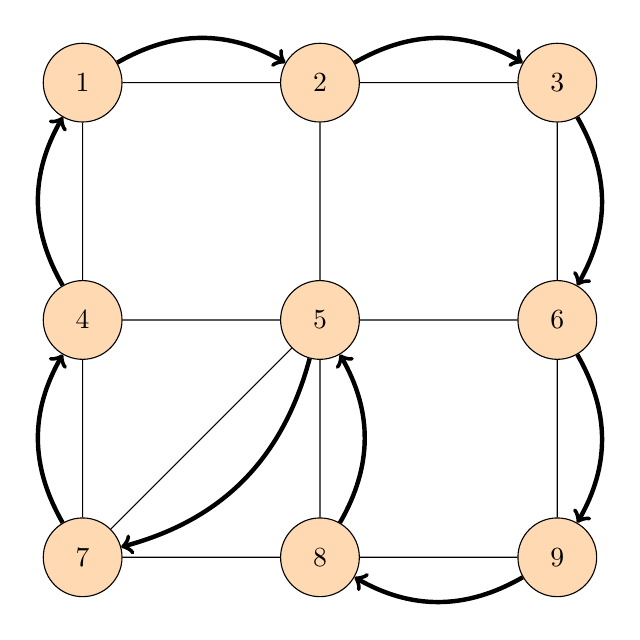
\begin{tikzpicture}
       \node[graph node] (1) {$1$};
       \node[graph node] (2) [right = 2cm of 1]{$2$};
       \node[graph node] (3) [right = 2cm of 2]{$3$};
       
       \node[graph node] (4) [below = 2cm of 1]{$4$};
       \node[graph node] (5) [right = 2cm of 4]{$5$};
       \node[graph node] (6) [right = 2cm of 5]{$6$};
       
       \node[graph node] (7) [below = 2cm of 4]{$7$};
       \node[graph node] (8) [right = 2cm of 7]{$8$};
       \node[graph node] (9) [right = 2cm of 8]{$9$};
       
       \draw
       (1) -- (2) -- (3)
       (1) -- (4) -- (7)
       (2) -- (5) -- (8)
       (3) -- (6) -- (9)
       (4) -- (5) -- (6)
(7) -- (8) -- (9)
       (7) -- (5);
	   
	   \draw [ultra thick,->,bend left=30] (1) to (2);
	   \draw [ultra thick,->,bend left=30] (2) to (3);
	   \draw [ultra thick,->,bend left=30] (3) to (6);
	   \draw [ultra thick,->,bend left=30] (6) to (9);
	   \draw [ultra thick,->,bend left=30] (9) to (8);
	   \draw [ultra thick,->,bend right=30] (8) to (5);
	   \draw [ultra thick,->,bend left=30] (5) to (7);
	   \draw [ultra thick,->,bend left=30] (7) to (4);
	   \draw [ultra thick,->,bend left=30] (4) to (1);	   	   	   	   	   	   
    \end{tikzpicture}
\end{center}

\pagebreak

\begin{center}
	\vspace*{-4cm}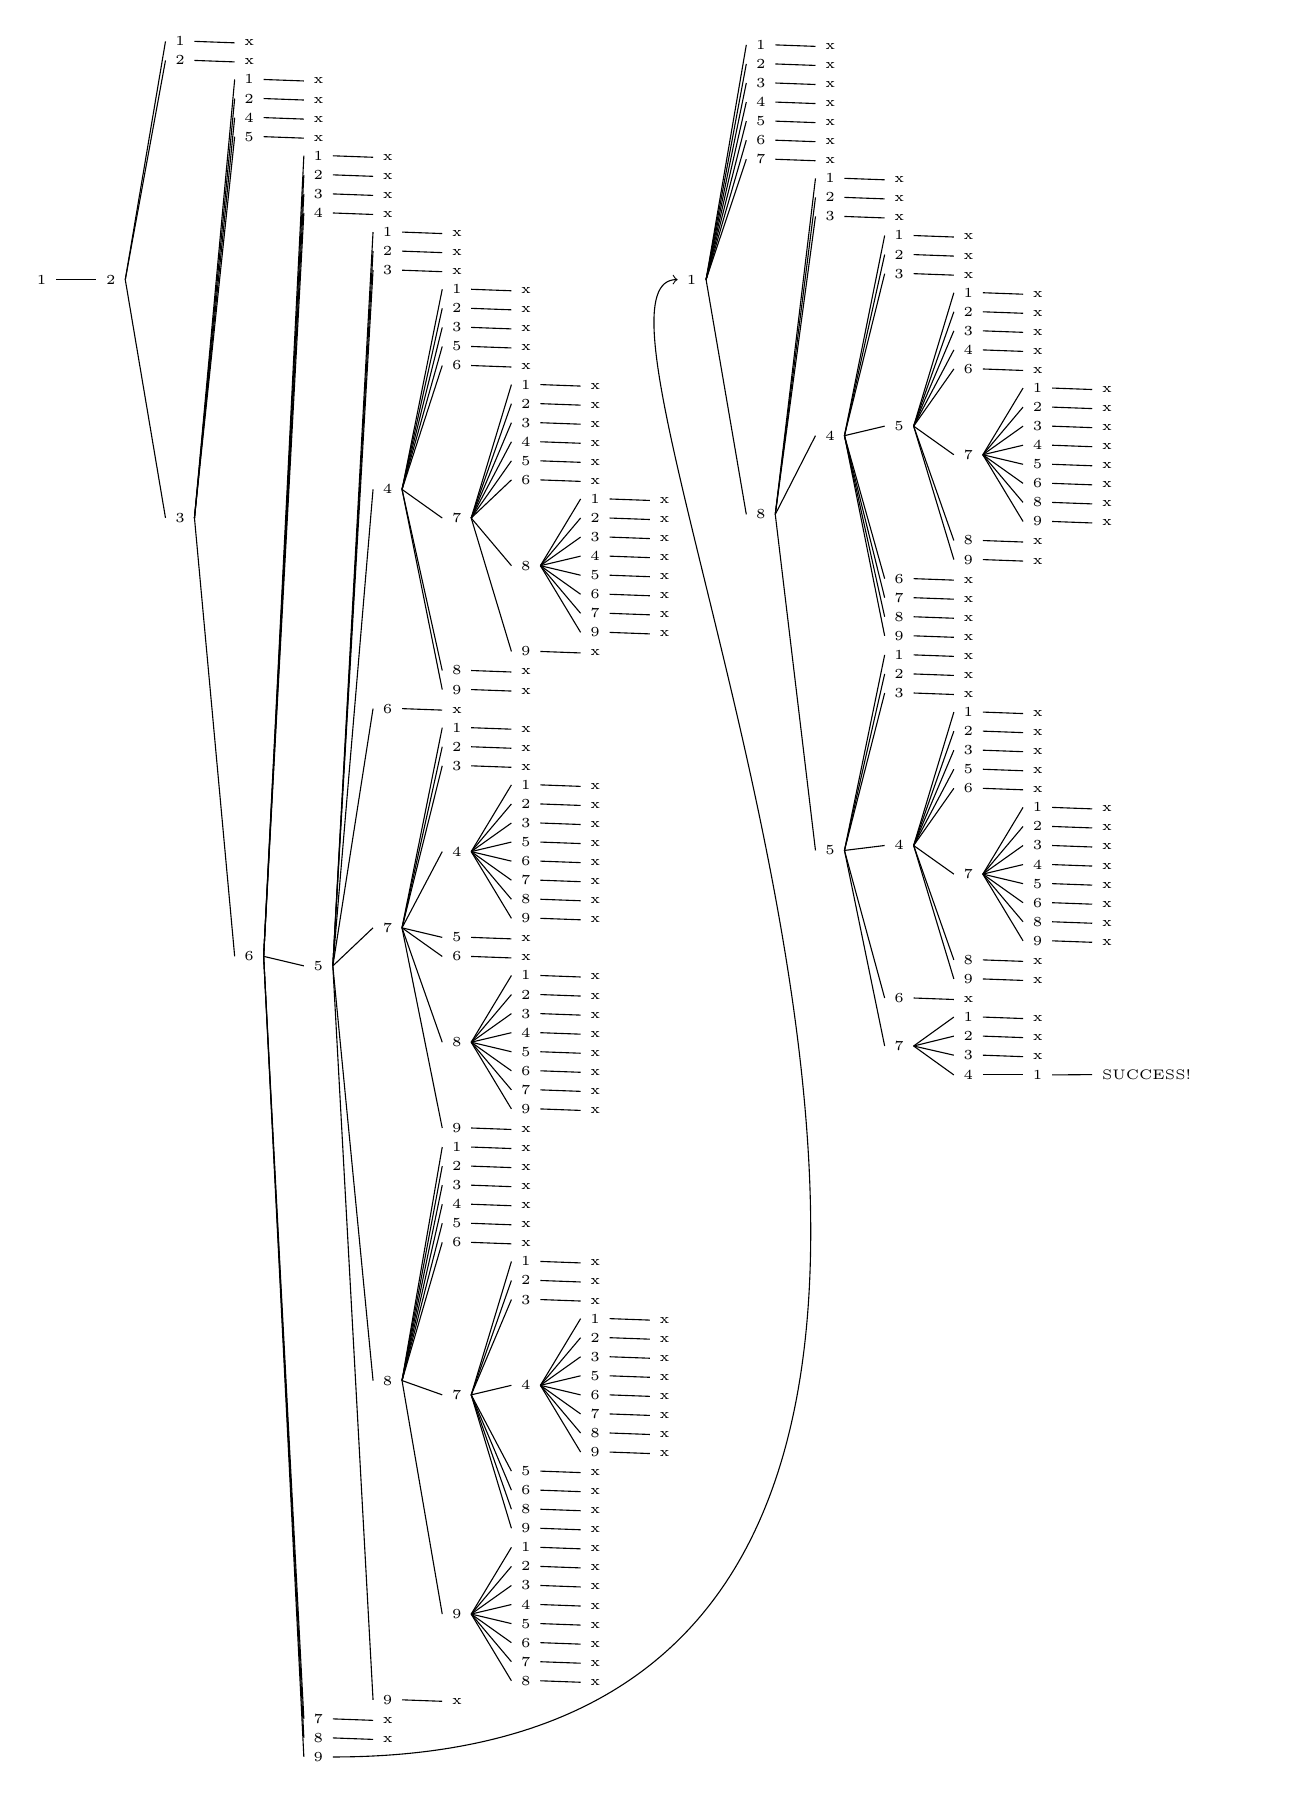
\begin{tikzpicture}[font=\tiny]
	\tikzset{grow'=right,level distance=25pt,sibling distance=-3pt}
%	\tikzset{execute at begin node=\strut}
	\tikzset{every tree node/.style={align=center,anchor=base west}}		

\Tree 
[.1 
	[.2 
		[.1 
			x
		] 
		[.2 
			x
		]
		[.3
			[.1
				x
			]
			[.2
				x
			]
			[.4
				x
			]
			[.5
				x
			]
			[.6
				[.1
					x
				]
				[.2
					x
				]
				[.3
					x
				]
				[.4
					x
				]
				[.5
					[.1
						x
					]
					[.2
						x
					]
					[.3
						x
					]
					[.4
						[.1
							x
						]
						[.2
							x
						]
						[.3
							x
						]
						[.5
							x
						]
						[.6
							x
						]
						[.7
							[.1
								x
							]
							[.2
								x
							]
							[.3
								x
							]
							[.4
								x
							]
							[.5
								x
							]
							[.6
								x
							]
							[.8
								[.1
									x
								]
								[.2
									x
								]
								[.3
									x
								]
								[.4
									x
								]
								[.5
									x
								]
								[.6
									x
								]
								[.7
									x
								]
								[.9
									x
								]
							]
							[.9
								x
							]
						]
						[.8
							x
						]
						[.9
							x
						]
					]
					[.6
						x
					]
					[.7
						[.1
							x
						]
						[.2
							x
						]
						[.3
							x
						]
						[.4
							[.1
								x
							]
							[.2
								x
							]
							[.3
								x
							]
							[.5
								x
							]
							[.6
								x
							]
							[.7
								x
							]
							[.8
								x
							]
							[.9
								x
							]
						]
						[.5
							x
						]
						[.6
							x
						]
						[.8
							[.1
								x
							]
							[.2
								x
							]
							[.3
								x
							]
							[.4
								x
							]
							[.5
								x
							]
							[.6
								x
							]
							[.7
								x
							]
							[.9
								x
							]
						]
						[.9
							x
						]
					]
					[.8
						[.1
							x
						]
						[.2
							x
						]
						[.3
							x
						]
						[.4
							x
						]
						[.5
							x
						]
						[.6
							x
						]
						[.7
							[.1
								x
							]
							[.2
								x
							]
							[.3
								x
							]
							[.4
								[.1
									x
								]
								[.2
									x
								]
								[.3
									x
								]
								[.5
									x
								]
								[.6
									x
								]
								[.7
									x
								]
								[.8
									x
								]
								[.9
									x
								]
							]
							[.5
								x
							]
							[.6
								x
							]
							[.8
								x
							]
							[.9
								x
							]
						]
						[.9
							[.1
								x
							]
							[.2
								x
							]
							[.3
								x
							]
							[.4
								x
							]
							[.5
								x
							]
							[.6
								x
							]
							[.7
								x
							]
							[.8
								x
							]
						]
					]
					[.9
						x
					]
				]
				[.7
					x
				]
			    [.8
					x
				]
			    [.\node(site){$9$}; ]
			]
		] 
	] 
]

\begin{scope}[shift={(3.25in,0in)}]
\Tree
[.\node(root){$1$}; 
	[.1
		x
	]
	[.2
		x
	]
	[.3
		x
	]
	[.4
		x
	]
	[.5
		x
	]
	[.6
		x
	]
	[.7
		x
	]
	[.8
		[.1
			x
		]
		[.2
			x
		]
		[.3
			x
		]
		[.4
			[.1
				x
			]
			[.2
				x
			]
			[.3
				x
			]
			[.5
				[.1
					x
				]
				[.2
					x
				]
				[.3
					x
				]
				[.4
					x
				]
				[.6
					x
				]
				[.7
					[.1
						x
					]
					[.2
						x
					]
					[.3
						x
					]
					[.4
						x
					]
					[.5
						x
					]
					[.6
						x
					]
					[.8
						x
					]
					[.9
						x
					]
				]
				[.8
					x
				]
				[.9
					x
				]
			]
			[.6
				x
			]
			[.7
				x
			]
			[.8
				x
			]
			[.9
				x
			]
		]
		[.5
			[.1
				x
			]
			[.2
				x
			]
			[.3
				x
			]
			[.4
				[.1
					x
				]
				[.2
					x
				]
				[.3
					x
				]
				[.5
					x
				]
				[.6
					x
				]
				[.7
					[.1
						x
					]
					[.2
						x
					]
					[.3
						x
					]
					[.4
						x
					]
					[.5
						x
					]
					[.6
						x
					]
					[.8
						x
					]
					[.9
						x
					]
				]
				[.8
					x
				]
				[.9
					x
				]
			]
			[.6
				x
			]
			[.7
				[.1
					x
				]
				[.2
					x
				]
				[.3
					x
				]
				[.4
					[.1
						SUCCESS!
					]
				]
			]
		]
	]
]
\end{scope}
\draw[<-](\subtreeof{root}.133.2) ..
controls +(west:2) and +(east:12)..(site);

	\end{tikzpicture}
\end{center}
	\section*{Problem 7}

In this problem we are asked to find a seating arrangement for 150 people at a 
round table such that no two people who dislike one another are forced to sit
adjacent to one another.
\\
\\
For each guest, we know the list of people they quarrel with. Thus, we can 
construct a graph where each node is a person on the guest list, and each edge
represets a person they do not quarrel with. We can determine the edges out of
each node by subtracting the list of people that the person the node represents
quarrels with from the guest list.
\\
\\
With this graph constructed, we then apply the algorithm for the 
\textit{Hamiltonian Circuit Problem} to find a circuit of the graph such that
each person is sitting next to someone they do not quarrel with.
\\
\\
Note: it is possible to construct a graph using these rules for which there is
no Hamiltonian Circuit. This occurs when there is no ordering of guests such
that only non-quarreling guests sit next to each other.

\end{document}